\documentclass{article}
% The LaTeX macro language is complicated, so we have inserted
% lots of documenting comments into the file.  Comments start
% with `%' and continue to the end of the line.  In Overleaf's
% window, they are colored green
%
% Comments prefixed with `Student:' are relevant to students.
% Skip anything else you don't understand, or ask me.
%
% set font encoding for PDFLaTeX or XeLaTeX
\usepackage{ifxetex}
\ifxetex
  \usepackage{fontspec}
\else
  \usepackage[T1]{fontenc}
  \usepackage[utf8]{inputenc}
  \usepackage{lmodern}
\fi

% Student: These lines describe some document metadata.
\title{Problem Set 6}
\author{%
% Student: change the next line to your name!
    Name
\\  MATH-UA 120 Discrete Mathematics
}
\date{due December 9, 2022 at 11:00pm}


\usepackage[headings=runin-fixed-nr]{exsheets}
% These make enumerates within questions start at the second ("(a)") level, rather than the first ("1.") level.
\makeatletter
    \newcommand{\stepenumdepth}{\advance\@enumdepth\@ne}
\makeatother
\SetupExSheets{
    question/pre-body-hook=\stepenumdepth,
    solution/pre-body-hook=\stepenumdepth,
}
\DeclareInstance{exsheets-heading}{runin-nn-np}{default}{
    runin = true,
    title-post-code = .\space,
    join = {
        main[r,vc]title[l,vc](0pt,0pt);
    }
}
\newif\ifshowsolutions
% Student: replace `false' with `true' to typeset your solutions.
% Otherwise they are ignored!
\showsolutionstrue
\ifshowsolutions
    \SetupExSheets{
        question/pre-hook=\itshape,
        solution/headings=runin-nn-np,
        solution/print=true,
        solution/name=Answer
    }%
    \makeatletter%
    \pretocmd{\@title}{Answers to }%
    \makeatother%
\else
    \SetupExSheets{solution/print=false}
\fi

% Bug workaround: http://tex.stackexchange.com/a/146536/1402
%\newenvironment{exercise}{}{}
\RenewQuSolPair{question}{solution}
%\let\answer\solution
%\let\endanswer\endsolution
\usepackage{manfnt}
\newcommand{\danger}{\marginpar[\hfill\dbend]{\dbend\hfill}}

% We are creating a command for some common commands.
\newcommand{\Z}{\mathbb{Z}}
\newcommand{\N}{\mathbb{N}}
\newcommand{\modulo}{\text{mod }}
\newcommand{\divisor}{\text{ div }}

% This package is for specifying graphics.  It's amazing.
% Manual at http://texdoc.net/texmf-dist/doc/generic/pgf/pgfmanual.pdf
\usepackage{tikz}
\tikzstyle{vertex}=[circle,draw,fill=none,inner sep=0pt,outer sep=0pt, minimum width=1ex]
\tikzstyle{edge}=[draw,thick]
\usepackage{multirow, multicol}
\usepackage{amsmath, amsthm}
\usepackage{amsfonts}
\usepackage{siunitx}
\DeclareSIUnit\pound{lb}
\usepackage{hyperref}
\newtheorem*{theorem}{Theorem}
\theoremstyle{definition}
\newtheorem*{definition}{Definition}
\newenvironment{note}{\noindent\emph{Note}.}{}
% This is the beginning of the part of the file that describes
% the text of the document.
% That's why it says `\begin{document}' below. :-)
\begin{document}
\maketitle



These are to be written up and turned in to Gradescope.\\



\ifshowsolutions
    \SetupExSheets{solution/print=true}
\else
    \danger
 \underline{ \LaTeX  Instructions:}  You can view the source (\texttt{.tex}) file to get some more examples of \LaTeX{} code.  I have commented the source file in places where new \LaTeX{} constructions are used.
  
  Remember to change \verb|\showsolutionsfalse| to \verb|\showsolutionstrue|
    in the document's preamble 
    (between \verb|\documentclass{article}| and \verb|\begin{document}|)
\fi

\section*{Assigned Problems}



\begin{question}
    (Scheinerman, Exercise 35.7:)
    What is wrong with the following statements?  Repair these statements and prove your revised versions.
    \begin{enumerate}
	\item For all integers $a, b$, we have $b |a$ iff  $a \divisor b = \frac{a}{b}$.
	\item For all integers $a, b$, we have $b|a$ iff $a \modulo b = 0$.
    \end{enumerate}
\end{question}
% Student: put your answer between the next two lines.
\begin{solution}
Alternatively we can extend the definition of div and mod so that $b$ can also be negative (if $b = 0$, $b|a$ is not true and neither $a \divisor b$ nor $a \modulo b$ would make sense, hence we do not need to worry about $b = 0$).

 Let us extend the definition of div and mod as follows:\\
 Suppose that $a, b \in \Z$ and $b \neq 0$.  There exists unique $q, r \in \Z$, {\color{blue}$0 \leq r < |b|$}, such that $a = bq + r$.  Then, we define: $a \modulo b = r$ and $a \divisor b = q$.
  
Then,\begin{enumerate}
	\item For all integers $a, b$ where $b\neq 0$, we have $b |a$ iff  $a \divisor b = \frac{a}{b}$.
	\item For all integers $a, b$ where $b \neq 0$, we have $b|a$ iff $a \modulo b = 0$.
	\begin{proof}  Suppose that $a, b \in \Z$.  Re-define $a \mod b$ and $a \divisor b$ as above.
	
	$(\Rightarrow)$ Suppose that $b|a$.  There exists some integer $n$ such that $a = bn$.  So, $a = bn + 0$ and $n = \frac{a}{b}$.  By the definition of div, $a \divisor b = n = \frac{a}{b}$ and $a \modulo b = 0$.
	
	Therefore, we have shown that if $b|a$ then $a \divisor b = \frac{a}{b}$ and $a \modulo b = 0$.
	
	$(\Leftarrow)$ Suppose that $a \divisor b = \frac{a}{b}$.  Since $a \divisor b$ must be an integer, then $\frac{a}{b} = n \in \Z$.  Therefore, $a = bn$ for this integer $n$.  By the definition of divisibility, $b | a$.
	
	Suppose that $a \modulo b = 0$.  By the definition of mod, this means that $a = bn + 0 = bn$ for some integer $n$.  By the definition of divisibility, $b | a$.
	\end{proof}
\end{enumerate}
\end{solution}

\begin{question}
    Find integers $a, b$ that do not have a greatest common divisor.  Prove that the pair of numbers that you found are the only pair of integers that do not have a gcd.
\end{question}
% Student: put your answer between the next two lines.
\begin{solution}
$a = 0, b =0$ is the only pair of integers that do not have a gcd.
\begin{proof}
We claim that $\gcd(0, 0)$ does not exist: Note that any integer $a \in \Z$ divides $0$.  Therefore, the set of common divisors of 0 and 0 is $\Z$, which does not have a largest element.  Therefore, $gcd(0, 0)$ does not exist.

Suppose that $a, b$ are any integers such that one of them is not zero.  Without loss of generality, suppose that $a \neq 0$.  This means that $a$ has finitely-many divisors and its greatest divisor is $a$ itself.  Furthermore, $a, b$ must have at least one divisor in common: the number 1 divides any number.  Thus, the gcd of $a$ and $b$ is the largest element of a nonempty and finite set of numbers (that are each $\leq a$); such a largest element must exist.  Therefore, $\gcd(a, b)$ exists.

Therefore, $0, 0$ is the only pair of integers that do not have a gcd.
\end{proof}
\end{solution}

\begin{question}
    (Scheinerman, Exercise 36.2:)
    For each pair of integers $a$ and $b$, find integers $x$ and $y$
    such that $ax+by = \gcd(a,b)$.
    \begin{enumerate}
        \item $\gcd(20,25)$
        \item $\gcd(0,10)$
        \item $\gcd(-89,-98)$
        \item $\gcd(123,-123)$
        \item $\gcd(54321,50)$
        \item $\gcd(1739,29341)$
    \end{enumerate}
\begin{note}
    You should do all of these for practice.
    But you only need to turn in (a), (c), and (e).
\end{note}
\end{question}
% Student: put your answer between the next two lines.
\begin{solution}
    \begin{enumerate}
        \item $\gcd(20,25) = 5$.  Since $5 = 25-20$, $x=-1$ and $y=1$ will do.
        \item $\gcd(0,10) = 10$.  Since $10 = 0 \times 10 + 1 \times 0$, $x=1$ and $y=0$ will work.
        \item $\gcd(-89,-98) = gcd(89,98) = gcd(98,89)$
            We use the Euclidean algorithm from here:
            \begin{align*}
                98 &= 1 \times 89 + 9 &\implies 9 &= 98 - 1 \times 89 \\
                89 &= 9 \times 9 + 8  &\implies 8 &= 89 - 9 \times 9 \\
                 9 &= 1 \times 8 + 1  &\implies 1 &= 9 - 1 \times 8
            \end{align*}
            So
            \begin{align*}
                1 &= 9 - 1 \times 8 \\
                  &= 8 - 1 \times (89 - 9 \times 9)
                   = 10 \times 9 - 1 \times 89 \\
                  &= 10 \times (98 - 1 \times 89) - 1 \times 89
                   = 10 \times 98 - 11 \times 89 \\
                  &= (-10) \times (-98) + 11 \times (-89)
            \end{align*}
            So $a=11$ and $b=-10$.
        \item $\gcd(123,-123) =123$, so $a=1$ and $b=0$.
        \item By the Euclidean algorithm:
            \begin{align*}
                54321 &= 1086 \times 50 + 21 &\implies 21 &= 54321 - 1086 \times 50 \\
                   50 &= 2 \times 21 + 8     &\implies 8  &= 50 - 2 \times 21 \\
                   21 &= 2 \times 8 + 5      &\implies 5  &= 21 - 2 \times 8 \\
                    8 &= 1 \times 5 + 3      &\implies 3  &=  8 - 1 \times 5 \\
                    5 &= 1 \times 3 + 2      &\implies 2  &=  5 - 1 \times 3 \\
                    3 &= 1 \times 2 + 1
            \end{align*}
            Therefore
            \begin{align*}
                1 &= 1\times 3 - 1 \times 2 \\
                  &= 1\times 3 - 1 \times (5 - 1 \times 3)
                   = 2 \times 3 - 1 \times 5 \\
                  &= 2 \times (8 - 1 \times 5) - 1 \times 5
                   = 2 \times 8 - 3 \times 5 \\
                  &= 2 \times 8 - 3 \times (21 - 2 \times 8)
                   = 8 \times 8 - 3 \times 21 \\
                  &= 8 \times (50 - 2 \times 21) - 3 \times 21
                   = 8 \times 50 - 19 \times 21 \\
                  &= 8 \times 50 - 19 \times (54321 - 1086 \times 50)
                   = 20642 \times 50 - 19 \times 54321
            \end{align*}
            So $a=-19$ and $b=20642$.
        \item One last time:
            \begin{align*}
                29341 &= 16 \times 1739 + 1517
                 &\implies 1517 &= 29341 - 16 \times 1739 \\
                 1739 &= 1 \times 1517 + 222
                 &\implies  222 &= 1739 - 1 \times 1517 \\
                 1517 &= 6 \times 222 + 185
                 &\implies  185 &= 1517 - 6 \times 222 \\
                  222 &= 1 \times 185 + 37
                  &\implies  37 &= 222 - 1 \times 185 \\
                  185 &= 5 \times 37 + 0
            \end{align*}
            So $\gcd(1739,29341) = 37$.  Working backwards,
            \begin{align*}
                37 &= 222 - 1 \times 185 \\
                   &= 222 - 1 \times (1517 - 6 \times 222)
                    = 7 \times 222 - 1 \times 1517 \\
                   &= 7 \times (1739 - 1 \times 1517) - 1 \times 1517
                    = 7 \times 1739 - 8 \times 1517 \\
                   &= 7 \times 1739 - 8 \times (29341 - 16 \times 1739)
                    = 135 \times 1739 - 8 \times 29341
            \end{align*}
            So $a=135$ and $b=-8$.
    \end{enumerate}
\end{solution}

\begin{question}
    (Scheinerman, Exercise 36.12:) 
    Let $a$ be an integer.  Prove that $2a+1$ and $4a^2+1$ are relatively prime.
\end{question}
% Student: put your answer between the next two lines.
\begin{solution}
\begin{proof}[Proof 1:]
To show that $2a+1$ and $4a^2 + 1$ are relatively prime, it is sufficient to show that there are integers $m, n$ such that
\[ m(2a+1) + n(4a^2+1) = 1. \]
Let $m = 2a^2 - a +1$ and $n = -a$.  Check that
\[  (2a^2 - a +1)(2a+1) -a(4a^2+1) = 1.  \]
\end{proof}

\begin{proof}[Proof 2:]
    Let $d = \gcd(2a+1,4a^2+1)$.
    Writing
    \[
        (4a^2+1)\times 1 + (2a+1)\times (1-2a) = 4a^2 + 1 + 1 - 4a^2 = 2
    \]
    we see that $d \mid 2$.  Since $d>0$, the only cases are $d=1$ and $d=2$.
    However, both integers are odd, so $d \neq 2$.  Therefore $d=1$.
\end{proof}
\end{solution}


\begin{question}
    (Scheinerman, Exercise 36.20:)
    A class of $n$ children sit in a circle.
    The teacher walks around the outside of the circle and pats every
    $k$th child on the head.
    Find and prove a necessary and sufficient condition on $n$ and $k$
    for every child to receive a pat on the head.
\end{question}
% Student: put your answer between the next two lines.
\begin{solution}
    We claim that every child is patted on the head if and only $n$ and
    $k$ are relatively prime.

    Suppose that every child is patted on the head.  In particular,
    the person right next to the first person gets patted on the head.
    If this child is the $a$th child patted, and the teacher has
    made $b$ loops of the circle of children, then
    This means $ak = bn + 1$, or $ak-bn=1$.  Therefore $n$ and $k$
    are relatively prime.

    On the other hand, suppose $n$ and $k$ are relatively prime.
    Then there exist positive integers $a$ and $b$ such that $ak - bn = 1$,
    or $ak = bn+1$.  So the $a$th person patted on the head is the person
    right next to the first person.  The child next to that child is
    patted after $a$ more children.  In this fashion, every child
    gets patted on the head. 
\end{solution}

\begin{question}\label{q:ve}
     Let $G=(V,E)$ be a graph. Prove by induction: 
\begin{quote}
The sum of the degrees of the vertices in $G$ is twice the number of edges.
\end{quote}	
\end{question}
% Student: put your answer between the next two lines.
\begin{solution}
Let $G=(V,E)$ be a graph and $d$ be the sum of the degree of all the vertices of $G$. We will prove $d=2|E|$ by induction.
\begin{description}
\item[Basis:] Consider $|E|=0$. If there are no edges, then the degree of all vertices must be zero. Then $d=0$ and $2|E|=0$. Hence the statement is true for $|E|=0$.
\item[Inductive Hypothesis:] Consider $|E|=n$ for $n\in \N$. Assume that $d=2n$.
\item[Inductive Step:] Consider a graph $G=(V,E)$ with $|E|=n+1$. Let $e\in E$. If we remove the edge $e$ from the graph G, then we have the graph $G'=G-e$. Graph $G'$ has $n$ edges; hence, the sum of the degree of the vertices of $G'$ is $2n$. Since $e$ cannot be a loop, it must have two distinct endpoints. Then exactly two vertices in $G'$ has one degree less than their degree in $G$. Then the sum of the degrees of the vertices of $G'$ is two less than the sum of the degrees of the vertices of $G$. So the sum of the degrees of the vertices of $G$ is $2n+2=2(n+1)$.
Therefore, by the principal of mathematical induction, the statement is true.
\end{description}
\end{solution}

\begin{question}
    (Scheinerman, Exercise 47.15:)
    Let $G$ be a graph. Prove that there must be an even number of vertices of odd degree.
\end{question}
% Student: put your answer between the next two lines.
\begin{solution}
Note: Vertices of even degree contribute an even amount to the sum in Question \ref{q:ve}. Therefore, vertices of odd degree must also contribute an even amount to the sum in Question \ref{q:ve}.
\begin{proof}
For the sake of contradiction, suppose there are an odd number of vertices of odd degree in $G$. Then they would contribute an odd amount to the sum of the degree of all vertices in $G$. However, by Question \ref{q:ve}, we know the sum of the degree of all vertices is twice the number of edges, which makes the sum even by definition. Contradiction! Therefore, there must be an even number of vertices of odd degree.
\end{proof} 
\end{solution}

\begin{question}
    Suppose $G$ is a subgraph of $H$.  Prove or disprove:
\begin{enumerate}
	\item $\alpha(G) \leq \alpha(H)$
	\item $\omega(G) \leq \omega(H)$
	\end{enumerate}
\end{question}
% Student: put your answer between the next two lines.
\begin{solution}
\begin{enumerate}
	\item False: The independence number (the size of the largest independent set) of a subgraph can be larger than the independence number of a graph.

Consider $H = K_3$, the complete graph on 3 vertices.  Since any two vertices are adjacent, the size of the largest independent set is 1.  So, $\alpha(H)= 1$.

Let $G$ be the subgraph of $H$ that contains no edge: $V(G) = \{1, 2, 3\}$ and $E(G) = \{ \}$.  Then, $\alpha(G) = 3 > \alpha(H)$.

	\item True: The clique number (the size of the largest clique) of a subgraph is less than or equal to the clique number of a graph.

\begin{proof}
Suppose that $G$ is a subgraph of $H$.  This means that $V(G) \subseteq V(H)$ and $E(G) \subseteq E(H)$.

Suppose that $\omega(G) = k$, for some $k \in \Z$, positive.  This means that there are $k$ vertices $v_1, \ldots, v_k \in V(G) \subseteq V(H)$ such that any two of them are adjacent in $G$; that is, $\{v_i, v_j \} \in E(G) \subseteq E(H)$.

This means that $v_1, \ldots, v_k$ also form a clique in $H$.  So, $H$ has a clique of size $k$.  This means that $\omega(H) \geq k = \omega(G)$.

Therefore, we have shown that $\omega(G) \leq \omega(H)$.
\end{proof}
\end{enumerate}
\end{solution}


\begin{question}
    (Scheinerman, Exercise 47.21:)
    Let  $G$ and $H$ be graphs.  We say that $G$ is \emph{isomorphic} to $H$
    provided there is a bijection $f \colon V(G) \to V(H)$ such that
    for all $a,b \in V(G)$ we have $a \sim b$ (in $G$) if and only if $f(a) \sim
    f(b)$ (in $H$).  The function $f$ is called an \emph{isomorphism} of $G$ to
    $H$.  We can think of $f$ as renaming the vertices of $G$ with the names of
    the vertices in $H$ in a way that preserves adjacency.  Less formally,
    isomorphic graphs have the same drawing (except for the names of the
    vertices).
    \begin{enumerate}
        \item Prove that isomorphic graphs have the same number of vertices.
        \item Prove that  if $f \colon V(G) \to V(H)$ is an
            isomorphism of graphs $G$ and $H$ and if $v \in V(G)$, then the
            degree of $v$ in $G$ equals the degree of $f(v)$ in $H$.
        \item Prove that isomorphic graphs have the same number of edges.
        \item Give an example of two graphs that have the same number of
            vertices and same number of edges but are not isomorphic.
        \item Let $G$ be the graph whose vertex set is $\{ 1,2,3,4,5,6\}$.  In
            this graph, there is an edge from $v$ to $w$ if and only if $v-w$ is
            odd.  Let $H$ be the graph below.  Find an
            isomorphism $f \colon V(G) \to V(H)$.
    \end{enumerate}
    \begin{center}
    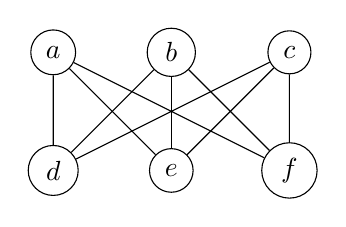
\begin{tikzpicture}[
        every node/.append style={draw,circle}
    ]
        \node (A) at (-1.5, 0) {$a$};
        \node (B) at (0, 0)    {$b$};
        \node (C) at (1.5, 0)  {$c$};
        \node (D) at (-1.5, -1.5) {$d$};
        \node (E) at (0, -1.5)   {$e$};
        \node (F) at (1.5, -1.5) {$f$};
        \draw (A) -- (D) -- (C) -- (F) -- (A);
        \draw (A) -- (E) -- (C);
        \draw (D) -- (B) -- (F);
        \draw (B) -- (E);
    \end{tikzpicture}
    \end{center}
\end{question}
% Student: put your answer between the next two lines.
\begin{solution}
    \begin{enumerate}
        \item  Let  $G$ and $H$ be isomorphic graphs.  Then $f \colon V(G) \to
            V(H)$ is a bijection.  It  follows that $|V(G)| = |V(H)|$.  Thus
            isomorphic graphs $G$ and $H$ have the same number of vertices.

        \item Let $f \colon V(G) \to V(H)$ be an isomorphism of
            graphs $G$ and $H$.  Suppose $v \in V(G)$.  By the definition of
            graph isomorphism, we have that
            \begin{align*}
                \deg_G(v) &= |\{w \in V(G) : w \sim v\}|
                        \\&= |\{f(w) \in V(H) : f(w) \sim f(v)\}| = \deg_H(v).
            \end{align*}
            Thus, the degree of $v$ in $G$ equals the degree of $f(v)$ in $H$.

        \item Let $f \colon V(G) \to V(H)$ be an isomorphism of
            graphs $G$ and $H$.  Suppose $v \in V(G)$.  By the definition of
            graph isomorphism, we know from (b) that
            \begin{align*}
                |E(G)| &= \frac{1}{2}\sum_{v \in V(G)} \deg_G(v)
                    \\&= \frac{1}{2}\sum_{f(v) \in V(H)} \deg_H(f(v)) = |E(H)|.
            \end{align*}
            Thus, isomorphic graphs have the same number of edges.

        \item Consider two graph $G$ and $H$ where $V(G) = V(H) = \{1,2,3,4\}$
            and
            \[
                E(G) = \{ \{1,2\}, \{2,3\}, \{3,4\}, \{4,1\} \}
            \]
            and
            \[
                E(H) =  \{ \{1,2\}, \{2,3\}, \{3,1\}, \{4,1\} \}
            \]
            Clearly $G$ and $H$ have the same number of vertices and edges. On
            the other hand, each vertex in $G$ has degree $2$ while vertex $1$
            in $H$ has degree $3$. Then, by part (b), the two graphs can not be
            isomorphic.

        \item Such an isomorphism is given, for example, by $f$ defined as
            \begin{align*}
                f(1) &= a, \quad f(2) = e, \quad f(3) = c
            \\  f(4) &= d, \quad f(5) = b, \quad f(6) = f
            \end{align*}
    \end{enumerate}
\end{solution}

\begin{question}\label{Sch-48-10}
    (Scheinerman, Exercise 48.10:) Let $G = (V,E)$
    be a graph on with $V = \left\{1,2,3,4,5,6\right\}$.  In
    Figure~\ref{fig-Sch-48-10} we show the graphs $G-1$, $G-2$, and so on but we
    do not show the names of the vertices.
        \begin{figure}\centering
        \begin{tabular}{ccc}
            $G-1$ & $G-2$ & $G-3$ \\
            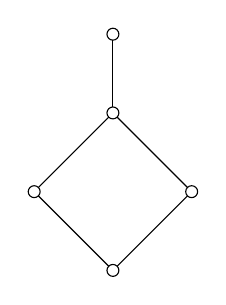
\begin{tikzpicture}
                 \path node[vertex] (A) {}
                     ++ ( 0,-1) node[vertex] (B) {} edge (A)
                     ++ (-1,-1) node[vertex] (C) {} edge (B)
                     ++ ( 1,-1) node[vertex] (D) {} edge (C)
                     ++ ( 1, 1) node[vertex] (E) {} edge (D) edge (B);
            \end{tikzpicture}
            &
            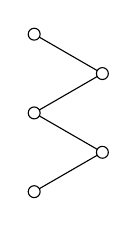
\begin{tikzpicture}
                 \path node[vertex] (A) {}
                     ++ (-30:1) node[vertex] (B) {} edge (A)
                     ++ (-150:1) node[vertex] (C) {} edge (B)
                     ++ (-30:1) node[vertex] (D) {} edge (C)
                     ++ (-150:1) node[vertex] (E) {} edge (D)
                     ;
            \end{tikzpicture}
            &
            \begin{tikzpicture}
                \path node[vertex] (A) {}
                    ++ (0,-1) node[vertex] (B) {} edge (A)
                    ++ (0,-1) node[vertex] (C) {} edge (B)
                    ++ (-1,-1) node[vertex] (D) {} edge (C)
                    ++ (2,0) node[vertex] (E) {} edge (C)
                    ;
            \end{tikzpicture}
            \\[3ex]
            $G-4$ & $G-5$ & $G-6$ \\
            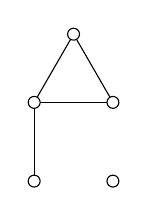
\begin{tikzpicture}
                \path node[vertex] (A) {}
                    ++ (1,0) node[vertex] (B) {} edge (A)
                    ++ (0,-1) node[vertex] (C) {}
                    ++ (-1,0) node[vertex] (D) {} edge (A)
                    (A) ++ (60:1) node[vertex] (E) {} edge (A) edge (B)
                    ;
            \end{tikzpicture}
            &
            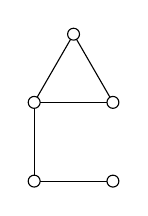
\begin{tikzpicture}
                \path node[vertex] (A) {}
                    ++ (1,0) node[vertex] (B) {} edge (A)
                    ++ (0,-1) node[vertex] (C) {}
                    ++ (-1,0) node[vertex] (D) {} edge (C) edge (A)
                    (A) ++ (60:1) node[vertex] (E) {} edge (A) edge (B)
                    ;
            \end{tikzpicture}
            &
            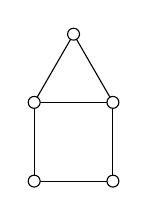
\begin{tikzpicture}
                \path node[vertex,
                    ] (A) {}
                    ++ (1,0) node[vertex,
                    ] (B) {} edge (A)
                    ++ (0,-1) node[vertex,
                    ] (C) {} edge (B)
                    ++ (-1,0) node[vertex,
                    ] (D) {} edge (C) edge (A)
                    (A) ++ (60:1) node[vertex,
                    ] (E) {} edge (A) edge (B)
                    ;
            \end{tikzpicture}
        \end{tabular}
        \caption{$G$ with each of its vertices deleted (Question~\ref{Sch-48-10})}
        \label{fig-Sch-48-10}
    \end{figure}
    The goal of this problem is to reconstruct the original graph $G$. Please do:
    \begin{enumerate}
        \item Determine the number of edges on $G$.
        \item Using your answer to (a), determine the degree of each of the six vertices of $G$.
        \item Determine $G$.
    \end{enumerate}
\end{question}
% Student: put your answer between the next two lines.
\begin{solution}
    \begin{enumerate}
        \item In the six graphs shown, each edge of $G$ appears \emph{four}
        times.  This is because each edge is incident on two vertices,
        so it gets deleted exactly twice.  Therefore the sum of the edge numbers
        of each of the six graph is four times the edge number of $G$:
        \[
            4 |E(G)| = \sum_{i=1}^6 |E(G-i)| = 28
        \]
        Therefore $|E(G)| = 7$.

        \item Since $|E(G-i)| = |E(G)| - d_G(i)$ for each $i$, we can solve
        \begin{table}
            \centering
            \begin{tabular}{>$c<$|>$c<$|>$c<$}
                i & |E(G-i)| & d_G(i) \\\hline
                1 & 5 & 2 \\
                2 & 4 & 3 \\
                3 & 4 & 3 \\
                4 & 4 & 3 \\
                5 & 5 & 2 \\
                6 & 6 & 1
            \end{tabular}
            \caption{Edge numbers and degrees (Question~\ref{Sch-48-10})}
            \label{tab-Sch-48-10}
        \end{table}
        for each $d_G(i)$.  The answers are in Table~\ref{tab-Sch-48-10}.

        \item We know that vertex $6$ is adjacent to only one other vertex.  By
        comparing the degrees of the vertices of $G$ and $G-6$, we see it must
        be adjacent to one of the vertices of degree $2$ in $G-6$, labeled $c$,
        $d$, or $e$.  If $6$ were adjacent to $e$, then $G-e$ would have one
        component like a square (four-cycle) and one isolated vertex.  That
        doesn't match any of the given graphs.  On the other hand, if $6$ were
        adjacent to $c$, then $G-c$ would resemble $G-4$, $G-d$ would resemble
        $G-5$, $G-b$ would resemble $G-2$, $G-a$ would resemble $G-3$, and
        $G-e$ would resemble $G-1$.  So this is a solution: $a=3$, $b=2$, $c=4$,
        $d=5$, $e=1$.

        we can name the other vertices
        $e=1$, $a=3$, $b=2$, $c=2$, and $d=5$.  The recovered $G$ is in
        Figure~\ref{fig-Sch-48-10-finished}.
        \begin{figure}
            \centering
            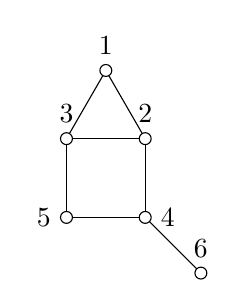
\begin{tikzpicture}
                \path node[vertex,label=$3$] (A) {}
                    ++ (1,0) node[vertex,label=$2$] (B) {} edge (A)
                    ++ (0,-1) node[vertex,label=right:$4$] (C) {} edge (B)
                    ++ (-1,0) node[vertex,label=left:$5$] (D) {} edge (C) edge (A)
                    (A) ++ (60:1) node[vertex,label=$1$] (E) {} edge (A) edge (B)
                    (C) ++ (-45:1) node[vertex,label=$6$] {} edge (C)
                    ;
            \end{tikzpicture}
            \caption{The recovered $G$ (Question~\ref{Sch-48-10})}
            \label{fig-Sch-48-10-finished}
        \end{figure}
    \end{enumerate}
\end{solution}



\end{document}
